\documentclass[12pt]{article}

\usepackage{fullpage}
\usepackage{multicol,multirow}
\usepackage{tabularx}
\usepackage{ulem}
\usepackage[utf8]{inputenc}
\usepackage[russian]{babel}
\usepackage{amsmath}
\usepackage{amssymb}
\usepackage{graphicx}
\usepackage{hyperref}

\newcommand{\quotes}[1]{"#1"}


\usepackage{titlesec}

\titleformat{\section}
  {\normalfont\Large\bfseries}{\thesection.}{0.3em}{}

\titleformat{\subsection}
  {\normalfont\large\bfseries}{\thesubsection.}{0.3em}{}

\titlespacing{\section}{0pt}{*2}{*2}
\titlespacing{\subsection}{0pt}{*1}{*1}
\titlespacing{\subsubsection}{0pt}{*0}{*0}
\usepackage{listings}
\lstloadlanguages{Lisp}
\lstset{extendedchars=false,
	breaklines=true,
	breakatwhitespace=true,
	keepspaces = true,
	tabsize=2
}
\begin{document}


\section*{Отчет по лабораторной работе №\,5
по курсу \guillemotleft  Функциональное программирование\guillemotright}
\begin{flushright}
Студент группы 8О-307 МАИ \textit{Спиридонов Кирилл}, \textnumero 18 по списку \\
\makebox[7cm]{Контакты: {\tt vo-ro@list.ru} \hfill} \\
\makebox[7cm]{Работа выполнена: 15.05.22 \hfill} \\
\ \\
Преподаватель: Иванов Дмитрий Анатольевич, доц. каф. 806 \\
\makebox[7cm]{Отчет сдан: \hfill} \\
\makebox[7cm]{Итоговая оценка: \hfill} \\
\makebox[7cm]{Подпись преподавателя: \hfill} \\

\end{flushright}

\section{Тема работы}
{\large Обобщённые функции, методы и классы объектов. \par}

\section{Цель работы}
{\large Научиться определять простейшие классы, порождать экземпляры классов, считывать и изменять значения слотов, научиться 
определять обобщённые функции и методы\par}

\section{Задание (вариант №5.39)}
{\large 
Определить обычную функцию line-intersections, принимающий один аргумент - список отрезков 
(экземпляров класса line). Причём концы отрезков могут задаваться как в 
декартовых (экземплярами cart), так и в полярных координатах (экземплярами polar).
\\
Функция должна возвращать список всех точек взаимного пересечения отрезков между собой.
\\
Результирующие точки могут быть получены либо в декартовых, либо в полярных 
координатах - на усмотрение выполняющего задание. Точки пересечения отрезков 
за их границами (как пересечения прямых) должны быть исключены из результирующего списка.
\\
"Вырожденные" случаи: параллельность, взаимное наложение и т.п. - следует исключить 
из рассмотрения и считать, что такого во входных данных не бывает.

(setq lines (list (make-instance 'line \\
                   :start (make-instance 'cart-или-polar ...) \\
                   :end (make-instance 'cart-или-polar ...)) \\
                  ...)) \\
\\
(line-intersections lines) \\
=> (cart-или-polar1 ...) \\
}

\section{Оборудование студента}
{\large Процессор Intel(R) Core(TM) i5-8250U CPU @ 1.60GHz, память: 8192Gb, разрядность системы: 64.}

\section{Программное обеспечение}
{\large ОС Ubuntu 20.04 LTS, среда LispWorks Personal Edition 7.1.2}

\section{Идея, метод, алгоритм}
{\large 
Идея алгоритма простая. Для начала необходимо определить, пересекаются ли отрезки. 
Необходимое и достаточное условие пересечения, которое должно быть соблюдено для 
обоих отрезков следующее: конечные точки одного из отрезков должны лежать в 
разных полуплоскостях, если разделить плоскость линией, на которой лежит второй из отрезков.
Так как все вектора лежат на плоскости X-Y, то их векторное произведение будет 
иметь ненулевой только компоненту Z, соответственно и отличие произведений векторов 
будет только в этой компоненте. Поэтому мы можем умножить попарно-векторно вектор 
разделяющего отрезка на векторы направленные от начала разделяющего отрезка к обеим точкам проверяемого отрезка. 
Если компоненты Z обоих произведений будет иметь различный знак, значит один из 
углов меньше 0 но больше -180, а второй больше 0 и меньше 180, соответственно 
точки лежат по разные стороны от прямой. Если компоненты Z обоих произведений имеют 
одинаковый знак, следовательно и лежат они по одну сторону от прямой.
Затем нам необходимо повторить операцию для другого отрезка и прямой, и убедиться 
в том, что расположение его конечных точек также удовлетворяет условию.
Если оказалось, что отрезки пересекаются, то из концов одного из отрезков опускаем 
перпендикуляры на другой отрезок. Там у нас получаются подобные треугольники. И 
отсюда находим координаты: \\
Px = Cx + (Dx-Cx)*|Z1|/|Z2-Z1|; \\
Py = Cy + (Dy-Cy)*|Z1|/|Z2-Z1|; \\

}

\section{Сценарий выполнения работы}

\section{Распечатка программы и её результаты}

\subsection{Исходный код}
\lstinputlisting{./lab5.lisp}

\subsection{Результаты работы}
% \lstinputlisting{./log2.lisp}

{\large 
	Результат выводиться в виде (list i j ans ...), где i и j номера отрезков в исходном списке, 
	поданном на вход, ans - точка, в которой эти отрезки пересекаются в декартовой системе координат. Так же
	для наглядности я прикрепил картнинки. \\

(setq lines (list (make-instance 'line \\
                   :start (make-instance 'cart :x 1 :y 4) \\
                   :end (make-instance 'cart :x 4 :y 1)) \\
					(make-instance 'line \\
                   :start (make-instance 'cart :x 1 :y 1) \\
                   :end (make-instance 'cart :x 4 :y 3)) \\
					(make-instance 'line \\
                   :start (make-instance 'cart :x 1 :y 2) \\
                   :end (make-instance 'cart :x 3 :y 4)) \\
					)) \\
([ОТРЕЗОК [CART x 1 y 4][CART x 4 y 1]] [ОТРЕЗОК [CART x 1 y 1] [CART x 4 y 3]] [ОТРЕЗОК [CART x 1 y 2] [CART x 3 y 4]]) \\

CL-USER 35 : 1 >  
(line-intersections lines) \\
(0 1 [CART x 14/5 y 11/5] 0 2 [CART x 2 y 3])

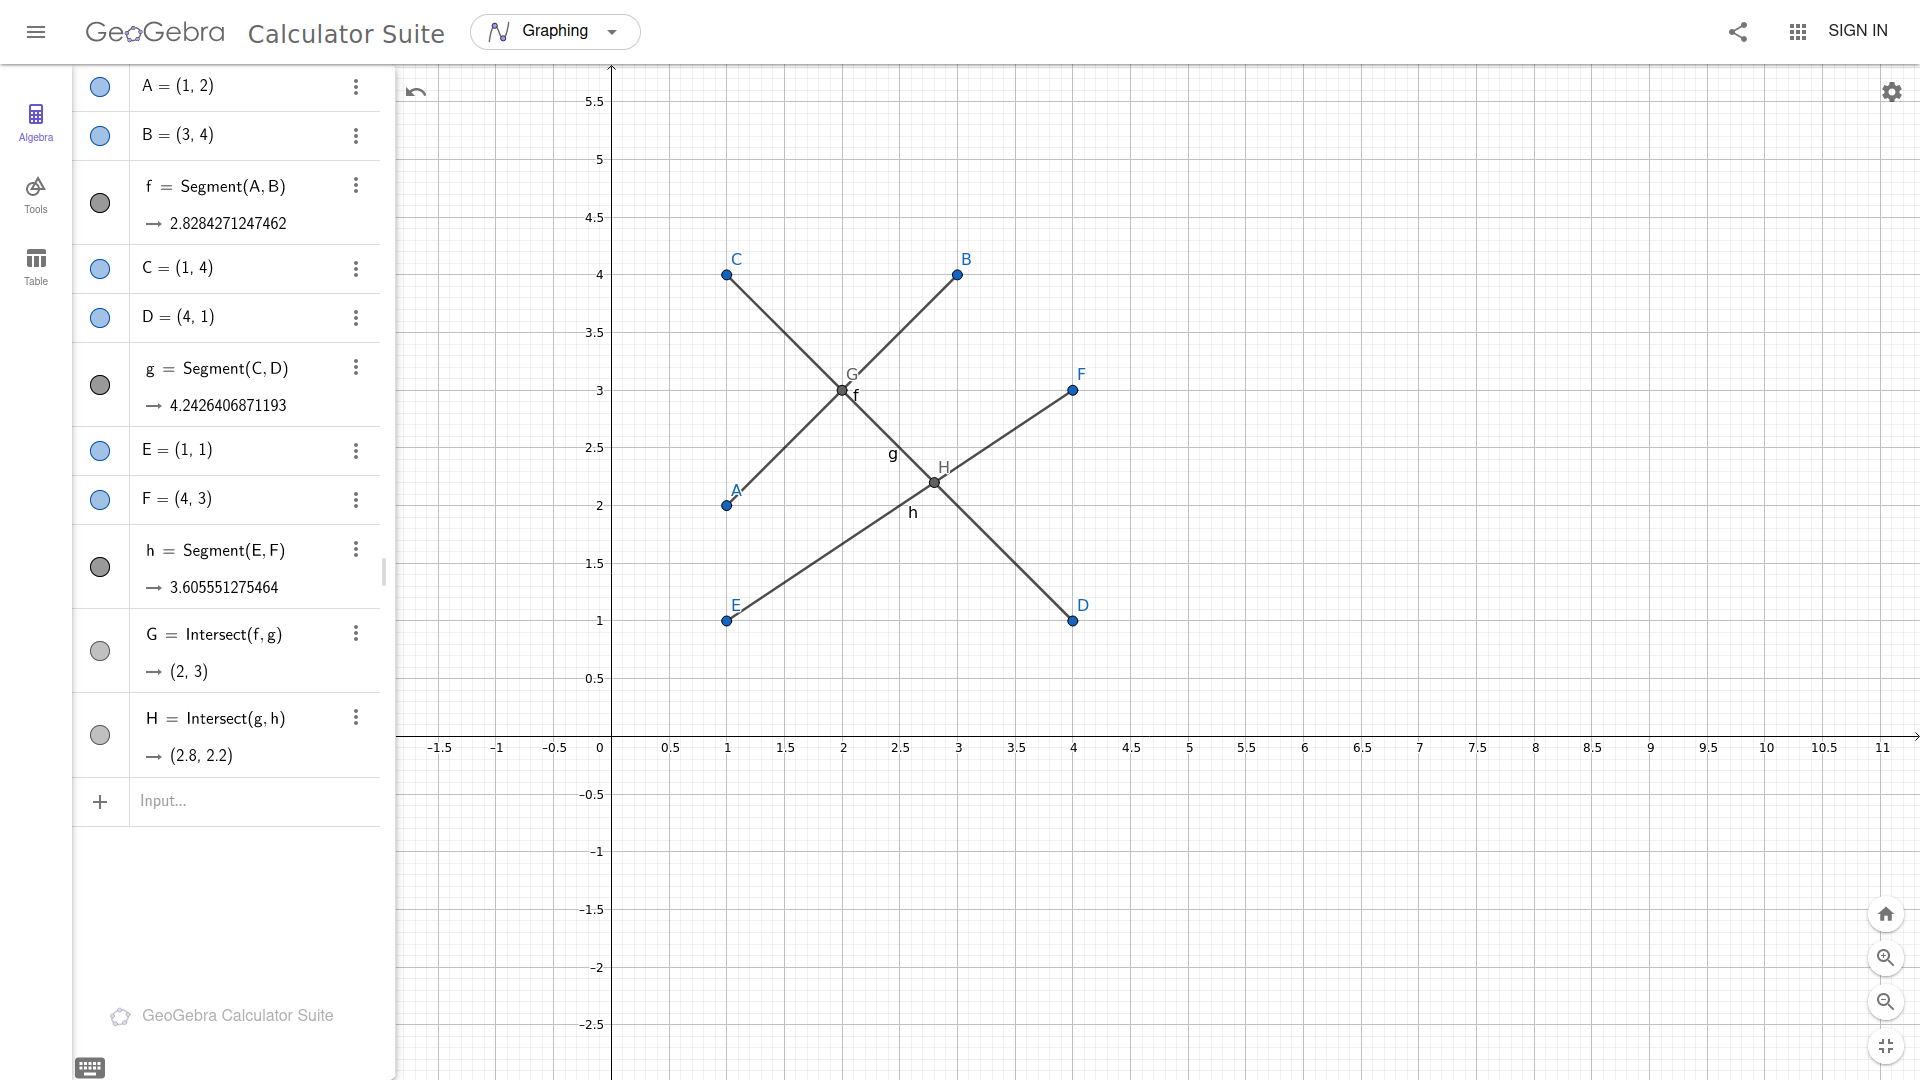
\includegraphics[scale=0.3]{1.png}

(setq lines (list (make-instance 'line \\
                   :start (make-instance 'polar :radius 10 :angle 2.094) \\
                   :end (make-instance 'polar :radius 12 :angle 2.792)) \\
					(make-instance 'line \\
                   :start (make-instance 'cart :x -14 :y 9) \\
                   :end (make-instance 'polar :radius 6 :angle 1)) \\
					(make-instance 'line \\ 
                   :start (make-instance 'cart :x 0 :y 4) \\
                   :end (make-instance 'cart :x 4 :y 10)) \\
					)) \\
([ОТРЕЗОК [POLAR radius 10 angle 2.094] [POLAR radius 12 angle 2.792]] [ОТРЕЗОК [CART x -14 y 9] [POLAR radius 6 angle 1]] [ОТРЕЗОК [CART x 0 y 4] [CART x 4 y 10]]) \\

CL-USER 27 > 
(line-intersections lines) \\
(0 1 [CART x -6.804698 y 7.3511076] 1 2 [CART x 1.0361822 y 5.5542736]) \\

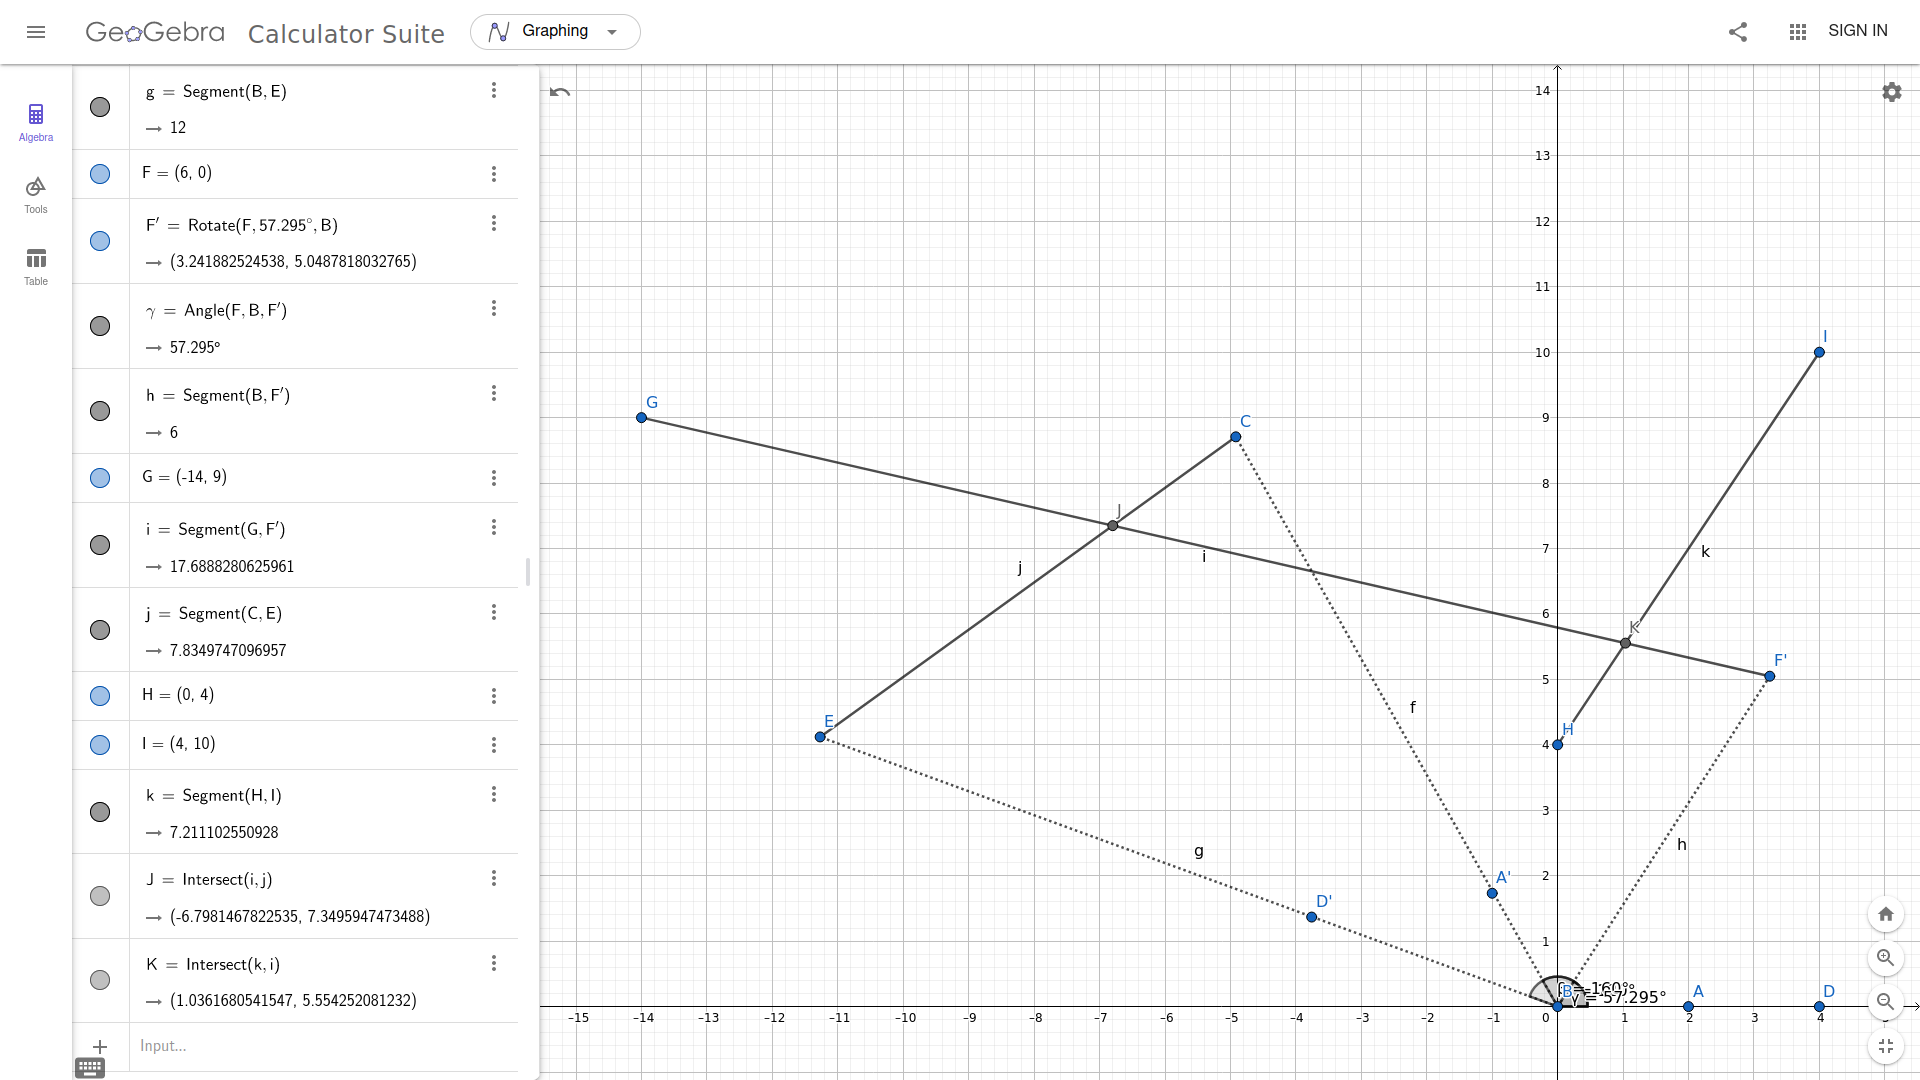
\includegraphics[scale=0.25]{2.png}

}

\section{Дневник отладки}
\begin{tabular}{|c|c|c|c|}
\hline
Дата & Событие & Действие по исправлению & Примечание \\
\hline
\end{tabular}

\section{Замечания автора по существу работы}
{\large 
	Вначале я хотел находить прямые, на которых лежат эти отрезки и по уравненияем 
	этих прямых смотреть, пересекаются ли они. Но наткнулся в интернете на алгоритм
	выше и решил попробовать реализовать его.
	Общая сложность алгоритма $O(n^2)$, т.к. каждый отрезок проверяется со всеми остальными.
}

\section{Выводы}
{\large 
	В данной лабораторной работе я научился определять простейшие классы, порождать
	экземпляры классов, считывать и изменять значения слотов в Common Lisp. 
	Так же в ходе выполнения лабораторной работы познакомился с новым алгоритмом
	для определения пересечения отрезков.
}
\end{document}
